\documentclass[a4paper,11pt]{article}
\usepackage[utf8]{inputenc}
\usepackage[T1]{fontenc}
\title{Universidade Federal do Rio Grande do Norte\\Métodos Computacionais em Engenharia - T01\linebreak\linebreak\linebreak Resolução Numérica de Equações Diferencias Parciais}
\author{}
\date{}
\usepackage{amsmath}
\usepackage{float}
\usepackage{ae}
\usepackage[brazil]{babel}
\usepackage{indentfirst}
\usepackage{url}
\usepackage{graphicx}
\usepackage[autostyle]{csquotes}
\graphicspath{ {./images/} }
\usepackage{hyperref}
\usepackage{verbatim}
\usepackage{minted}
\makeindex
%%%
%%%
\begin{document}
\maketitle
\thispagestyle{empty}
\vspace{2cm}
\begin{minipage}{\textwidth}
\flushright
{\large
Discente:\\
Alan Lima de Medeiros\\
\vspace{0.5cm}
\vspace{0.5cm}
Docente:\\
Paulo Sérgio da Motta Pires\\}
\vspace{7cm}
\center
{\large
Natal-RN\\04/2022}
\end{minipage} 

\tableofcontents

\pagebreak

\section{Introdução}
    O presente relatório tem como objetivo descrever duas formas de resolução de um problema de Dirichlet mediante a um exemplo. Um problema de Dirichlet constitui-se da obtenção de uma função, especificada para uma região com valores de contorno definidos, que seja capaz de solucionar uma equação diferencial parcial (EDP). 
    
    Neste contexto, apenas a EDP de Laplace será trabalhada via aproximações numéricas. Para tal, entende-se que a discretização do operador laplaciano ($\nabla^2$) permite encontrar uma solução aproximada para valores de pontos em uma determinada região, uma vez que a discretização transforma a EDP em uma equação de diferenças.
    
    Para se aplicar esse discretização do laplaciano, precisa-se discretizar também a região, determinando pontos dentro dela e estabelecendo distâncias $h_n$ entre eles. Feita essa malha, pode-se aplicar um gabarito, como o apresentado na figura \ref{gabarito}, e se obter as equações em cada ponto a partir da equação discretizada do laplaciano, equação \ref{eq:1}.
    
    \begin{figure}[H]
        \centering
        \makebox[\textwidth]{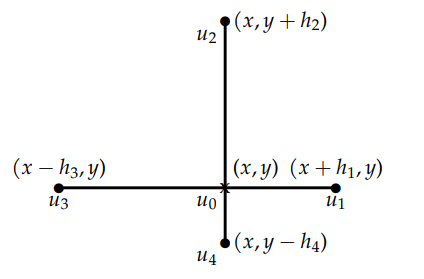
\includegraphics[scale=0.8]{images/gabarito.png}}
        \caption[width=\columnwidth]{Gabarito aplicado em uma malha não uniforme.}
        \label{gabarito}
    \end{figure}
    
    \begin{eqnarray}
        \label{eq:1}
        \nabla^2 = -2(\frac{1}{h_1h_3} + \frac{1}{h_2h_4})u_0 + \frac{2}{h_1(h_1+h_3)}u_1 + \frac{2}{h_2(h_2+h_4)}u_2 +\\\nonumber+ \frac{2}{h_3(h_3+h_1)}u_3 + \frac{2}{h_4(h_2+h_4)}u_4
    \end{eqnarray}

    Contudo, para o cenário deste projeto, será considerada apenas uma região com malha uniforme, ou seja, $h_1=h_2=h_3=h_4=h$. Desse modo, a equação \ref{eq:1} pode ser modificada para a forma apresentada na equação \ref{discreto}.
    
    \begin{eqnarray}
        \nabla^2 = -2(\frac{2}{h^2})u_0 + \frac{2}{2h^2}u_1 + \frac{2}{2h^2}u_2 + \frac{2}{2h^2}u_3 + \frac{2}{2h^2}u_4 \nonumber
    \end{eqnarray}
    \begin{eqnarray}
        \label{discreto}
        \nabla^2 = \frac{1}{h^2}(-4u_0 + u_1 + u_2 + u_3 + u_4)
    \end{eqnarray}
    
    Por ser a equação de Laplace, entende-se que $\nabla^2=0$. Nesse sentido, a equação que será utilizada no desenvolvimento da questão será a apresentada na equação \ref{final}.
    
    \begin{eqnarray}
        \label{final}
        -4u_0 + u_1 + u_2 + u_3 + u_4 = 0
    \end{eqnarray}
    
\pagebreak

\section{Metodologia}
    O desenvolvimento deste projeto foi feito, basicamente, em cinco etapas principais: planejamento, resolução manual, implementação do código de programação, análise dos resultados e escrita deste relatório. Sendo assim, na primeira etapa, o problema foi reconhecido e diferentes formas de solução foram cogitadas, inclusive, nesse estágio a linguagem de programação Python na versão 3.7.13 foi escolhida. 
    
    Paralelo a isso, o ambiente de desenvolvimento também foi escolhido, sendo ele o Google Colab, devido as suas facilidades de modularização e documentação do código, bem como por sua agilidade em seu acesso e integralização com o armazenamento em nuvem do Google Drive.
    
    No momento da resolução manual, a questão foi trabalhada no papel, tendo sua estrutura de resolução montada, isto é, a numeração dos pontos, a obtenção da equações e a montagem do sistema linear foi feita. Ademais, um rascunho da lógica de programação foi realizada, estabelecendo algumas estratégias para converter aquilo construído no papel para a linguagem de programação.
    
    No próprio desenvolvimento do algoritmo já foram explicitadas algumas análises dos resultados, como a comparação de tempo na utilização de diferentes funções. A propósito, algumas bibliotecas foram importadas para a resolução da questão, sendo elas a Numpy, a Pandas, a Seaborn e a Matplotlib. A primeira teve como papel disponibilizar algumas funções matemáticas para o código, como a resolução de sistemas lineares e as últimas três foram exploradas na aplicação de conceitos de ciência de dados, construindo tabelas e gráficos, como o heatmap.
    
    Por fim, este material foi produzido com a ferramenta de produção de documentos LaTeX, dentro do ambiente Overleaf. Esse compilador foi escolhido, pois apresenta muito suporte na escrita do documento e resguardar as alterações de forma automática.
    
\pagebreak

\section{Problema}
    O problema em questão consiste em encontrar os potenciais nos pontos vermelhos da região apresentada na figura \ref{problema}. Cabe ressaltar que o problema se trata de uma malha uniforme, ou seja, o parâmetro \textit{h} é constante entre todos os pontos internos ao triângulo. Neste caso, observa-se que ele corresponderá a 0,125.
    \begin{figure}[H]
        \centering
        \makebox[\textwidth]{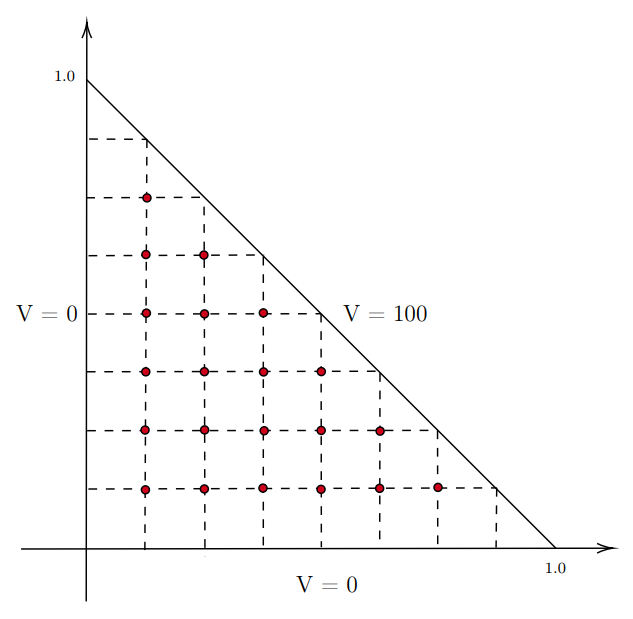
\includegraphics[scale=0.6]{images/Problema.png}}
        \caption[width=\columnwidth]{Região em estudo.}
        \label{problema}
    \end{figure}
    
    Além disso, deve-se levar em consideração que, em se tratando de um problema da equação de Laplace, as condições de contorno são valores bem definidos e não funções. Nesse sentido, as condições de contorno são:\\
        \[
        V=
        \begin{cases}
        0,&\mbox{se}\quad (x,y)\in{[(x,0) \cup (0,y)]},\\
        100, &\mbox{se}\quad (x,y)\in{y=x+1}.
        \end{cases}
        \]
        
    Diante do exposto, o problema solicita que os valores dos potenciais nos pontos internos do triângulo sejam encontrados por meio de dois algoritmos: pela obtenção e resolução do sistema linear que aproxima a solução da equação de Laplace e pelo método iterativo. Em seguida, pede ainda que seja feita uma análise comparativa entre as duas técnicas.
    
\subsection{Resolução: manual \label{manual}}
    A primeira forma escolhida de se resolver o problema foi a manual. A partir dessa resolução, se pôde confirmar, de forma redundante, os resultados obtidos nas demais seções, bem como auxiliou em seus processos de construção.
    
    A primeira etapa para se resolver manualmente é enumerar os pontos da malha e o padrão escolhido foi o observado na figura \ref{pontos}. Esse padrão será utilizado também nas demais seções. 
    
    \begin{figure}[H]
        \centering
        \makebox[\textwidth]{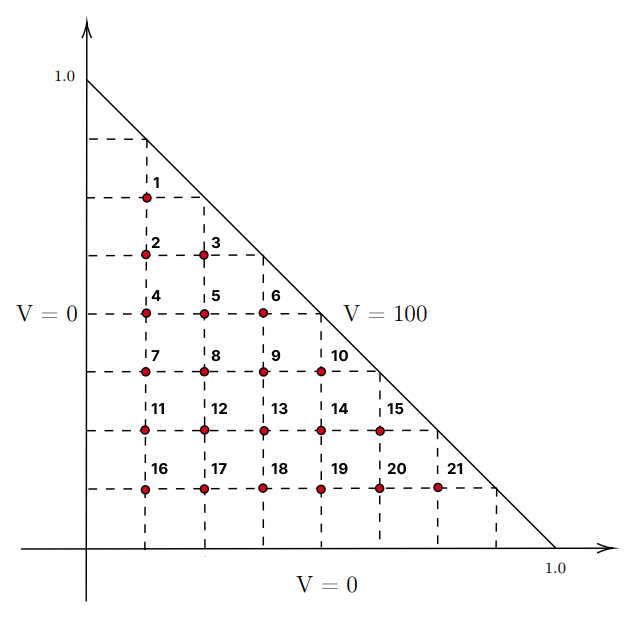
\includegraphics[scale=0.5]{images/Pontos.png}}
        \caption[width=\columnwidth]{Enumeração dos pontos.}
        \label{pontos}
    \end{figure}
    
    A partir dessa enumeração, pode-se aplicar o gabarito (ver figura \ref{discreto}) em cada ponto e encontrar a equação (ver equação \ref{final}) correspondente. Tomando o primeiro ponto como exemplo, tem-se:
    
    \begin{eqnarray}
        -4u_1 + u_2 + 100 + 100 + 0 = 0\nonumber
        \\
        -4u_1 + u_2 = -200\nonumber
    \end{eqnarray}
    
    Analogamente, todos os outros 21 pontos passarão por esse processo de equacionamento e, com isso, pode-se representar todas essas equações, que juntas formam um sistema linear, no formato $A_{21x21}u_{21x1}=b_{21x1}$, como observado abaixo:\\
    \begin{center}
    \begin{bmatrix}
    -4 & 1 & 0 & 0 & 0 & \cdots & 0 \\
    1 & -4 & 1 & 1 & 0 & \cdots & 0 \\
    \vdots & \vdots & \vdots & \vdots & \vdots & \ddots & \vdots \\
    0 & 0 & 0 & 0 & 0 & \cdots & -4 \\
    \end{bmatrix}
    \begin{bmatrix}
    u_1 \\
    u_2 \\
    \vdots \\
    u_{21} \\
    \end{bmatrix}
    =
    \begin{bmatrix}
    -200 \\
    0 \\
    \vdots \\
    -200 \\
    \end{bmatrix}
    \\
    \end{center}
    
    Utilizando uma calculadora de sistemas lineares online (matrixcalc), obteve-se como potenciais desses pontos os seguintes valores:
    \begin{center}
    \begin{bmatrix}
    u_1 \\
    u_2 \\
    u_3 \\
    u_4 \\
    u_5 \\
    u_6 \\
    u_7 \\
    u_8 \\
    u_9 \\
    u_{10} \\
    u_{11} \\
    u_{12} \\
    u_{13} \\
    u_{14} \\
    u_{15} \\
    u_{16} \\
    u_{17} \\
    u_{18} \\
    u_{19} \\
    u_{20} \\
    u_{21} \\
    \end{bmatrix}
    =
    \begin{bmatrix}
    60.25 \\
    41.02 \\
    74.26 \\
    29.55 \\
    56.02 \\
    79.04 \\
    21.18 \\
    41.23 \\
    60.13 \\
    79.04 \\
    13.93 \\
    27.58 \\
    41.23 \\
    56.02 \\
    74.26 \\
    6.97 \\
    13.93 \\
    21.18 \\
    29.55 \\
    41.02 \\
    60.25 \\
    \end{bmatrix}
    V
    \end{center}
    
\pagebreak

\subsection{Resolução: algoritmo da equação de Laplace \label{laplace}}
    A estratégia utilizada para transcrever a resolução arquitetada na seção \ref{manual} foi interpretar a região em questão como uma matriz. Desse modo, visando facilitar a compreensão e a manipulação computacional, completou-se a região triangular para se formar um quadrado. Seguidamente, estabeleceu-se que cada ponto de interseção entre as linhas tracejadas horizontais e verticais, incluindo as bordas, seria um elemento de uma matriz de ordem 9, figura \ref{matriz}.
    
    \begin{figure}[H]
        \centering
        \makebox[\textwidth]{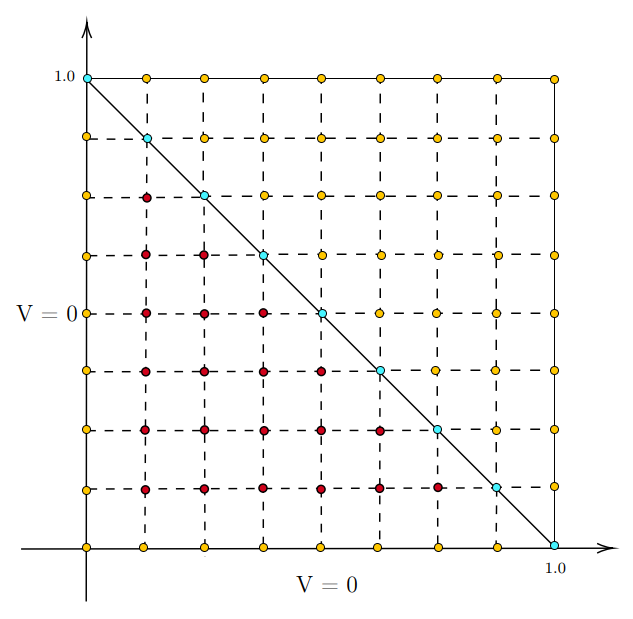
\includegraphics[scale=0.5]{images/Matriz_quadrada.png}}
        \caption[width=\columnwidth]{Completando o restante da matriz.}
        \label{matriz}
    \end{figure}
    
    Na figura \ref{matriz}, os pontos vermelhos representam os potenciais que devem ser encontrados, os amarelos onde o potencial é 0V e os azuis onde o potencial é 100V. Acima da diagonal principal, arbitrou-se 0V para todos os pontos, uma vez que, inicialmente, esses pontos não faziam parte do problema e isso facilitaria a solução, pois em Python já se pode iniciar uma matriz com valores 0.
    
    Para a solução foram declaradas duas matrizes: uma matriz quadrada de ordem 9, chamada de \textit{mpontos}, cuja função é enumerar os pontos vermelhos de 1 a 21, e outra matriz quadrada de ordem 21 para ser a matriz de coeficientes, \textit{A}. Além disso, um vetor de inteiros, \textit{b}, de 21 posições foi declarado para armazenar os termos independentes das equações. Sendo assim, tem-se o suficiente para resolver o sistema \textit{Ax=b}. Todas essas variáveis foram inicializadas com valores 0, como observado no trecho de código abaixo.

    \begin{minted}
        [
        frame=lines,
        framesep=2mm,
        baselinestretch=1.2,
        bgcolor=white,
        fontsize=\footnotesize,
        linenos
        ]
        {python}
import numpy as np

mpontos = np.zeros([9,9], dtype=float)  
A = np.zeros([21,21], dtype=int)      
b = np.zeros([21], dtype=int)                                         
    \end{minted}
    
    A matriz \textit{A} terá em cada linha os coeficientes presentes nas equações obtidas em cada ponto e cada coluna corresponderá a um ponto.  
    
    Para enumerar, criou-se um contador e se percorreu a matriz \textit{mpontos}, passando apenas pelos pontos vermelhos. Dessa maneira, nas linhas 5 e 6, estruturas condicionais fazem com que se ignore a primeira coluna, a última linha e todos os elementos acima da diagonal principal da matriz, incluindo a própria diagonal. Em outras palavras, ignoram os pontos definidos pelas condições de contorno. Nos pontos que respeitam essas condições, o valor de 0 na matriz é substituído pelo número do ponto e a variável contador é acrescida de 1 para continuar o processo, olhar o código abaixo.
    
    \begin{minted}
        [
        frame=lines,
        framesep=2mm,
        baselinestretch=1.2,
        bgcolor=white,
        fontsize=\footnotesize,
        linenos
        ]
        {python}
contador = 1

for i in range (0,9):
  for j in range (0,9):
    if(i != 8 and j != 0):            
      if(i>j):                        
        mpontos[i,j] = contador
        contador = contador + 1                                         
    \end{minted}
    
    Feita a enumeração dos pontos, deve-se agora percorrer esses pontos e aplicar o gabarito, discutido anteriormente. Todavia, as equações serão montadas indiretamente, haja vista que os valores dos coeficientes já serão postos na matriz \textit{A} e os termos independentes no vetor \textit{b}. Como se deseja apenas aplicar o gabarito nos pontos enumerados, a estrutura condicional da linha 3 do código abaixo faz com que se ignore todos os pontos da matriz \textit{mpontos} com valor 0 durante os laços.
    
    Na linha 4 do código abaixo, uma variável auxiliar receberá o número do ponto que se está aplicando o gabarito, desse modo, esse ponto corresponderá ao centro do gabarito. A variável \textit{aux} também será responsável por indicar qual linha da matriz de coeficientes deverá ser preenchida ao aplicar o gabarito nesse ponto central. 
    
    Na equação discretizada de Laplace, o ponto central recebe o coeficiente -4 e, por isso, na matriz \textit{A}, o valor de -4 será posto na linha e na coluna correspondente, lembrando sempre de subtrair 1 do auxiliar para acessar os elementos da matriz, tendo em vista que em Python os índices começam em 0. Portanto, o coeficiente de um determinado ponto de número n será sempre armazenado na matriz de coeficientes em uma coluna com índice n-1.
    
    \begin{minted}
        [
        frame=lines,
        framesep=2mm,
        baselinestretch=1.2,
        bgcolor=white,
        fontsize=\footnotesize,
        linenos
        ]
        {python}
for i in range (0,9):
  for j in range (0,9):
    if(mpontos[i,j]!=0):              
      aux = int(mpontos[i,j])         
      A[aux-1, aux-1] = -4            

      if(i==j+1):                     
        b[aux-1]=b[aux-1]-100
      else:                           
        var = int(mpontos[i,j+1])     
        A[aux-1, var-1] = 1

      if(j-1!=0):
        var = int(mpontos[i,j-1])
        A[aux-1, var-1] = 1

      if(j==i-1):
        b[aux-1]=b[aux-1]-100
      else:
        var = int(mpontos[i-1,j])
        A[aux-1, var-1] = 1
      
      if(i+1!=8):                 
        var = int(mpontos[i+1,j])
        A[aux-1, var-1] = 1                                     
    \end{minted}
    
    Para verificar os quatro outros pontos do gabarito, outras quatro estruturas condicionais são criadas das linhas 7 a 25. Na primeira condição, identifica-se o ponto da direita, cujas únicas possibilidades são de ser 100V (valor de contorno) ou um outro ponto enumerado. Se os índices do ponto à direita forem iguais, significará que o ponto está na diagonal principal e, assim, -100V é adicionado à posição dessa equação no vetor \textit{b}. Se os índices não forem iguais, significará que aquele ponto é um outro ponto enumerado e, por isso, o valor de 1 é adicionado na linha e na coluna adequada da matriz de coeficientes. A variável \textit{var} armazena o número do ponto e é utilizada como índice para se acessar a coluna correta em \textit{A}. A mesma lógica é utilizada para verificar o ponto de cima do gabarito, das linhas 17 a 21.
    
    A verificação dos pontos da esquerda e de baixo funciona de maneira similar. Para esses pontos, há somente duas possibilidades: ou são 0V ou são outros pontos enumerados. Sendo assim, visando otimizar o código, as estruturas condicionais desses dois pontos são mais simples, pois não há a necessidade de se acrescentar algo à \textit{b}. As condições desses pontos são feitas nas linhas 13 e 23, respectivamente, do código acima. Na 13, se o índice da coluna for diferente de 0 (condição de contorno), adiciona-se 1 a coluna da matriz \textit{A} que representa aquele ponto enumerado. Já na linha 23, a mesma ideia é utilizada, contudo, para quando a linha de baixo diferente de 8.
    
    Por último, os valores dos potenciais dos pontos vermelhos são obtidos utilizando o método \textit{linalg.solve()} da biblioteca Numpy e armazenados no vetor \textit{x}. Os parâmetros passados são a matriz \textit{A} e o vetor \textit{b}. Olhar o código abaixo.
    
    \begin{minted}
        [
        frame=lines,
        framesep=2mm,
        baselinestretch=1.2,
        bgcolor=white,
        fontsize=\footnotesize,
        linenos
        ]
        {python}
x = np.linalg.solve(A,b)                                       
    \end{minted}
    
    Em suma, pode-se esclarecer melhor com um exemplo. Nesse sentido, toma-se o ponto 1 da figura \ref{pontos} como exemplo. Seguindo os passos do código, a primeira ação a se fazer é verificar o número do ponto e em seguida preencher a matriz de coeficientes. Dessa forma, em sendo o primeiro ponto, se estabelece que a linha que será preenchida de \textit{A} será a 0, além disso, na coluna 0 dessa linha coloca-se o valor de -4 devido ao termo central. Em seguida, observa-se os pontos no entorno desse, começando pelo da direita, nota-se que deverá ser somado -100V no elemento de índice 0 do vetor \textit{b}. O mesmo se dá para o ponto acima do elemento central, totalizando -200V na primeira posição de \textit{b}. Para o elemento à esquerda, nada é feito, pois seu valor é 0. Já para o ponto abaixo, percebe-se que é o ponto 2, então, deve-se adicionar o valor 1 na coluna 1 da linha 0 da matriz \textit{A}. O processo se repete para todos os outros pontos e, no fim, com a matriz \textit{A} e o vetor \textit{b} preenchidos, usa-se a função do Numpy para se calcular os valores de \textit{x} do sistema \textit{Ax=b}. O código completo e comentado pode ser visto no Anexo A.
    
    Os valores armazenados em \textit{x} ainda foram colocados em dois formatos para melhorar a visualização dos resultados. A primeira forma foi colocando os valores em um formato similar à região apresentada na questão. Para isso, percorreu-se a matriz \textit{mpontos} colocando o valor de 100V na diagonal principal e trocando os números dos pontos por seus valores de potenciais. Esse tratamento é feito no código abaixo das linhas 1 a 10.
    
    \begin{minted}
        [
        frame=lines,
        framesep=2mm,
        baselinestretch=1.2,
        bgcolor=white,
        fontsize=\footnotesize,
        linenos
        ]
        {python}
for i in range(0,9):
  for j in range(0,9):

      if(i==j):
        mpontos[i,j]=100
      elif(i==8 or j==0):
        mpontos[i,j]=0
      elif(i>j):
        ponto = int(mpontos[i,j])
        mpontos[i,j] = x[ponto-1]
        
for i in range(1,8):
  print(" ")
  for j in range(1,9):
    if(i>=j):
      print(str(round(mpontos[i,j],2)), end=" ")
    \end{minted}
    
    A impressão feita entre as linhas 12 e 16 do código acima apresentam um resultado como o visto na figura \ref{resultados_1}.
    
    \begin{figure}[H]
        \centering
        \makebox[\textwidth]{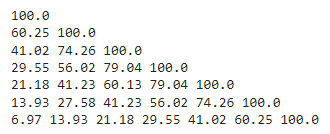
\includegraphics[scale=1]{images/resultado_1.png}}
        \caption[width=\columnwidth]{Impressão dos resultados obtidos.}
        \label{resultados_1}
    \end{figure}
    
    Por outro lado, uma outra forma de organização dos dados foi feita utilizando a biblioteca \textit{Pandas}. Com essa biblioteca, criou-se um dataframe com os valores organizados na matriz \textit{mpontos} na impressão anterior. Um dataframe em Python pode ser entendido, basicamente, como uma tabela visualmente mais agradável. O código para isso pode ser visto no trecho abaixo, além disso essa tabela pode ser visualizada na figura \ref{data_frame_1}.
    
    \begin{minted}
        [
        frame=lines,
        framesep=2mm,
        baselinestretch=1.2,
        bgcolor=white,
        fontsize=\footnotesize,
        linenos
        ]
        {python}
import pandas as pd

df = pd.DataFrame(mpontos)
df
    \end{minted}
    
    \begin{figure}[H]
        \centering
        \makebox[\textwidth]{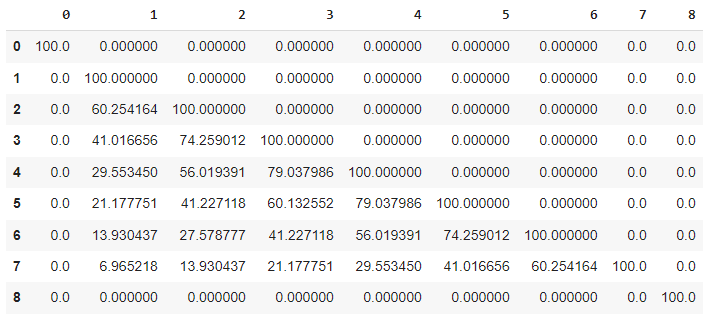
\includegraphics[scale=0.8]{images/data_frame_1.png}}
        \caption[width=\columnwidth]{Tabela feita com a biblioteca \textit{Pandas}.}
        \label{data_frame_1}
    \end{figure}
    
\pagebreak    
    
\subsection{Resolução: algoritmo iterativo}
    A resolução iterativa ainda segue o padrão observado na figura \ref{matriz}, entretanto, não se faz mais necessário montar as equações de cada ponto e, por conseguinte, o sistema linear. Por outro lado, alguns novos parâmetros aparecem: o valor inicial dos pontos vermelhos, a precisão dos potenciais e o número de repetições máximas. A biblioteca Numpy e a matriz quadrada de ordem 9 ainda são utilizadas.
    
    No trecho de código abaixo, pode-se observar a importação da biblioteca na primeira linha e, das linhas 3 a 5, a inicialização e leitura das novas variáveis. Vale salientar que para o chute inicial e a precisão, as variáveis foram estabelecidas como pontos flutuantes, porém o número de repetições máximas foi apontado como um inteiro, haja vista que, para esse contexto, não há frações de repetições. Por último, na linha 7, a matriz \textit{mpontos} representando a malha da figura \ref{matriz} é declarada com todos os potenciais sendo 0V pelos mesmos motivos explicados na seção anterior.
    
    \begin{minted}
        [
        frame=lines,
        framesep=2mm,
        baselinestretch=1.2,
        bgcolor=white,
        fontsize=\footnotesize,
        linenos
        ]
        {python}
import numpy as np

chute = float(input("Digite o chute inicial: "))            
precisao = float(input("Digite o valor da precisão: "))     
rep = int(input("Digite o número máximo de iterações: "))   

mpontos = np.zeros([9,9])                                   
    \end{minted}
    
    Na sequência, a matriz de pontos é percorrida substituindo os valores dos pontos internos da região pelo chute inicial e aplicando as condições de contorno. A otimização do código é de extrema relevância e, por isso, na linha 3 do código abaixo, o código ignora a última linha e a primeira coluna da matriz, tendo em vista que são valores de contorno iguais a 0V e a matriz já foi iniciada com 0V em todos os pontos. Outro tratamento é feito na linha 4, trocando os valores de todos os pontos abaixo da diagonal principal pelo valor do chute inicial e na linha 6, mudando os valores da diagonal principal de 0V para 100V.
    
    \begin{minted}
        [
        frame=lines,
        framesep=2mm,
        baselinestretch=1.2,
        bgcolor=white,
        fontsize=\footnotesize,
        linenos
        ]
        {python}
for i in range (0,9):
  for j in range (0,9):
    if(i != 8 and j != 0):      
      if(i>j):
        mpontos[i,j] = chute    
      elif(i==j):
        mpontos[i,j] = 100                                       
    \end{minted}
    
    Nesta técnica, o cálculo dos potenciais é parado de duas formas: ou a precisão em todos os pontos é satisfeita ou o número de repetições acabam. Sendo assim, no trecho do código abaixo, na linha 1 é declarada uma variável para controlar o cálculo da precisão. Logo abaixo, na linha 3, se estabelece uma estrutura de repetição que continuará funcionando enquanto a variável de controle tiver um valor booleano falso e o número de repetições não tiver acabado.
    
    \begin{minted}
        [
        frame=lines,
        framesep=2mm,
        baselinestretch=1.2,
        bgcolor=white,
        fontsize=\footnotesize,
        linenos
        ]
        {python}
stop = False                    

while((stop==False) and (rep!=0)):
  contador=0                                                                             

  for i in range (0,9):
    for j in range (0,9):
      if(i>j and i!=8 and j!=0):                                                         
        aux = mpontos[i,j]                                                               
        calculo = (mpontos[i,j+1]+mpontos[i,j-1]+mpontos[i+1,j]+mpontos[i-1,j])/4        
        mpontos[i,j]=calculo                                                             

        erro = abs((calculo-aux)/calculo)                                                
        if(erro<=precisao):
          contador = contador + 1                                                        
          if(contador == 21):                                                            
            stop = True
      
  rep = rep-1                                                                                                             
    \end{minted}
    
    Na linha 4, um contador é inicializado em 0, sendo ele responsável por contar quantos pontos já satisfazem à precisão estabelecida. Se esse contador chegar a 21, significará que todos os pontos satisfazem e o valor da variável \textit{stop} é mudado para verdadeiro, parando o cálculo. 
    
    Dentro da estrutura de repetição \textit{while}, percorre-se a matriz \textit{mpontos}, somente nos elementos que representam os pontos vermelhos e aplica-se o gabarito assim como na seção \ref{laplace}. Com o objetivo de se otimizar os cálculos, a obtenção do erro relativo é feito em cada ponto, assim que o novo valor do ponto é calculado. Desse modo, uma variável auxiliar, \textit{aux}, armazena o valor atual do ponto e a variável \textit{calculo} recebe o novo valor do ponto, seguindo a fórmula:
    
    \begin{equation}
        \label{eq:2}
        u_{i,j} =\frac{u_{i,j+1} + u_{i,j-1} + u_{i+1,j} + u_{i-1,j}}{4}
    \end{equation}
    
    O novo valor substitui o anterior na matriz \textit{mpontos} e, em mãos do valor anterior, guardado em \textit{aux}, e do novo valor, pode-se calcular o erro relativo. Se o erro relativo for menor ou igual à precisão, o contador é incrementado em 1 e, se chegar a 21, ativa-se o mecanismo de parada. No fim, o número de repetições é decrementado em 1 e o processo se repete até que alguma das condições de parada ocorra.
    
    Como exemplo, aplicando um chute inicial de 0V, uma precisão de 0.0001 e número máximo de repetições igual a 25, percebe-se que, com 2 casas decimais, os valores são iguais aos encontrados na seção \ref{laplace}. Para uma melhor visualização, os valores da matriz \textit{mpontos} foram organizados, novamente, em um dataframe, figura \ref{data_frame_2}. O algoritmo completo e comentado pode ser visto no Anexo B.
    
    \begin{figure}[H]
        \centering
        \makebox[\textwidth]{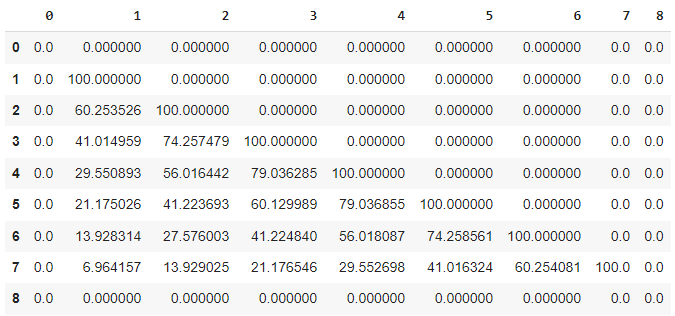
\includegraphics[scale=0.8]{images/data_frame_2.png}}
        \caption[width=\columnwidth]{Tabela feita com a biblioteca \textit{Pandas}.}
        \label{data_frame_2}
    \end{figure}
\pagebreak

\section{Conclusões}
    
    A resolução do mesmo problema de três maneiras diferentes garante uma redundância que aumenta o grau de certeza do resultado encontrado. Como os resultados coincidiram, pode-se representar de maneira gráfica os potenciais calculados. Desse modo, foi-se desenvolvido um \textit{heatmap} com as bibliotecas \textit{seaborn} e \textit{matplotlib} para se apresentar, visualmente, a variação do potencial na região. O código abaixo faz a construção do gráfico e ele pode ser visto na figura \ref{heatmap}.
        \begin{minted}
        [
        frame=lines,
        framesep=2mm,
        baselinestretch=1.2,
        bgcolor=white,
        fontsize=\footnotesize,
        linenos
        ]
        {python}
import seaborn as sns
import matplotlib.pyplot as plt
sns.set();

x = sns.heatmap(df, cmap='Reds');
plt.title('Heatmap da variação da tensão')
plt.show()                                                                                                         
    \end{minted}
    
    \begin{figure}[H]
        \centering
        \makebox[\textwidth]{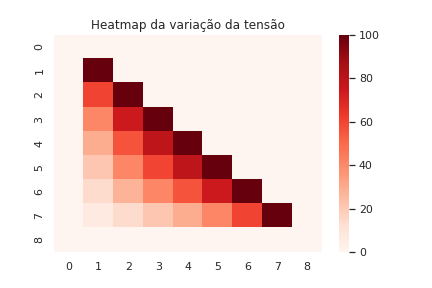
\includegraphics[scale=0.8]{images/Heatmap2.png}}
        \caption[width=\columnwidth]{Heatmap com h=1/8.}
        \label{heatmap}
    \end{figure}
    
    Como a discretização da região foi feita com um \textit{h} relativamente alto, o gráfico da figura acima tem uma aparência "pixelada". Para se ter uma ideia de algo mais contínuo, pode-se reduzir a distância \textit{h} e, consequentemente, aumentar a quantidade de potenciais calculados. Assim, ampliou-se a matriz de ordem 9 para uma de ordem 100, resultando em 4753 pontos internos ao invés de apenas 21. O \textit{heatmap} produzido foi o mostrado na figura \ref{heatmap100}.
    
    \begin{figure}[H]
        \centering
        \makebox[\textwidth]{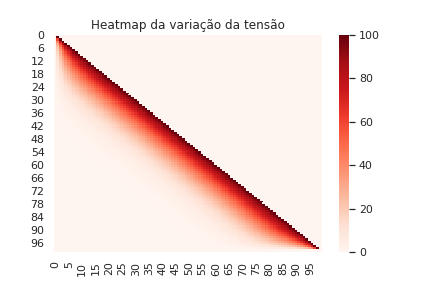
\includegraphics[scale=0.8]{images/Heatmap1.png}}
        \caption[width=\columnwidth]{Heatmap com 10000 pontos.}
        \label{heatmap100}
    \end{figure}
    
    A partir da análise do gráfico, nota-se que os resultados obtidos fazem sentido, pois quanto mais próximo da diagonal principal, mais próximo dos 100V.
    
    Outra análise feita foi a comparação entre os 3 métodos de resolução. A solução manual, quando comparada às outras duas, apresenta muitas limitações que acabam deixando-a em desvantagem. Esse tipo de solução está sujeita a muitas falhas humanas, bem como dispende muito tempo para ser utilizada. Diante disso, ela se torna altamente imprecisa e aplicável somente para regiões com poucos pontos.
    
    Por outro lado, comparando a resolução de Laplace e o método iterativo, observa-se que para regiões com muitos pontos, a solução iterativa será muito mais rápida, uma vez que não necessita montar equações e, nem tão pouco, preencher matrizes de coeficientes e de termos independentes. Ademais, o método iterativo não necessita utilizar técnicas de triangularização de matrizes para solucionar sistemas lineares, evitando - inclusive - erros matemáticos em processos de inversão de matrizes quando o determinante da matriz de coeficientes for 0, por exemplo.
    
    Para se comprovar essas afirmações, foram feitos gráficos comparando o tempo de execução dos métodos de Laplace e iterativo. Desse modo, o resultado obtido foi o apresentado na figura \ref{tempo}, mostrando que, para malhas pequenas (poucos pontos), os métodos são basicamente equivalentes quanto ao tempo, todavia, ao aumentar o número de pontos, o tempo do método de Laplace é muito maior que pelo outro método. 
    
    \begin{figure}[H]
        \centering
        \makebox[\textwidth]{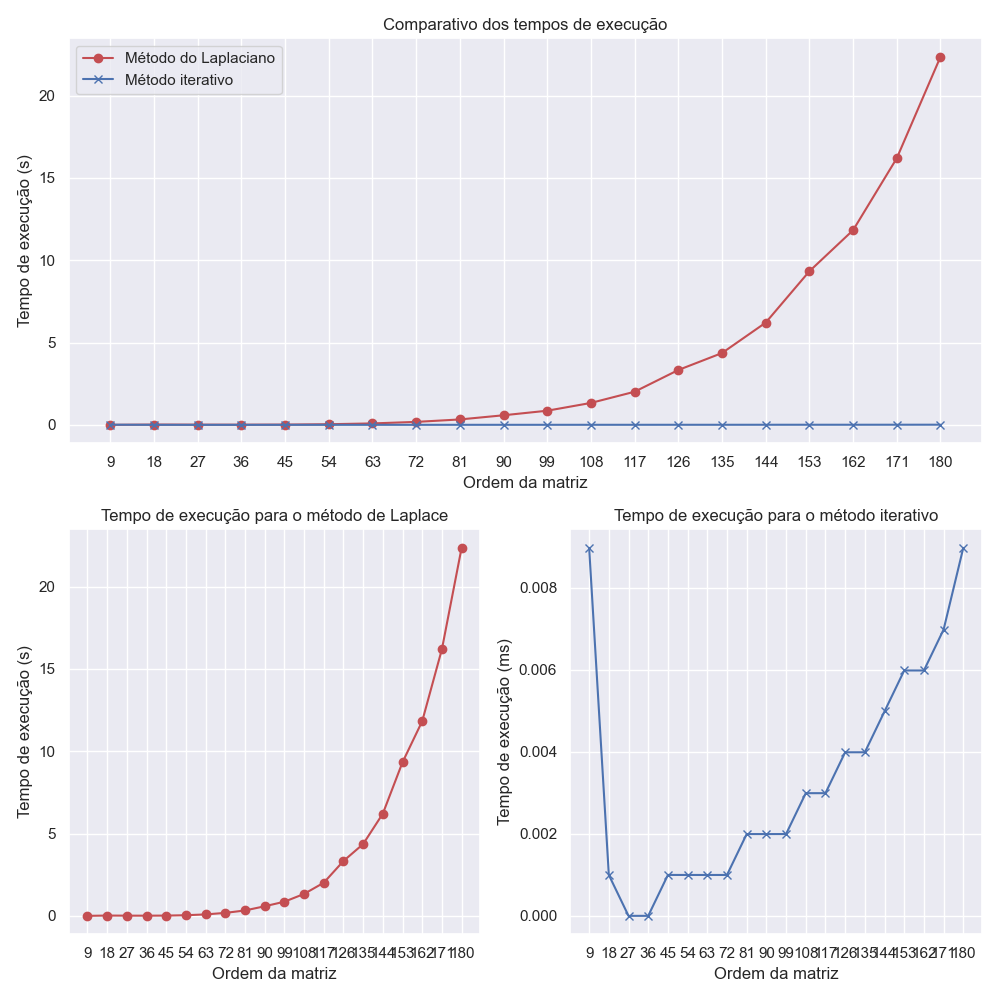
\includegraphics[scale=0.5]{images/Tempo.png}}
        \caption[width=\columnwidth]{Gráficos de tempo de execução.}
        \label{tempo}
    \end{figure}
    
    Os gráficos acima foram feitos variando a ordem das matrizes de 9 em 9, partindo de uma matriz 9 por 9. As matrizes aumentaram de tamanho até atingir um valor de 20 amostras.
    
    Por fim, para melhor analisar os códigos citados e os gráficos gerados, pode-se acessar o ambiente de desenvolvimento em: \url{https://colab.research.google.com/drive/11gISD-86ug4aCtMtmOyC6qLwfOXUAHSd?usp=sharing} e executar as células na ordem. A execução fora do ambiente virtual pode ser feita localmente, necessitando apenas da instalação manual das bibliotecas \textit{pandas, matplotlib, numpy e seaborn}.

\pagebreak

\section*{Referências}
\addcontentsline{toc}{section}{Referências}

Overleaf. \textbf{LaTeX documentation}. Disponível em:<\url{https://pt.overleaf.com/learn}>. Acesso em: 23 de abril de 2022.\\

Pandas. \textbf{pandas.DataFrame}. Disponível em:<\url{https://pandas.pydata.org/docs/reference/api/pandas.DataFrame.html}>. Acesso em: 23 de abril de 2022.\\

PIRES, Paulo. \textbf{Notas de aula - versão 0.21}. 2022.\\

SCHNEIDER, Felipe. \textbf{Como resolver sistemas lineares no Python.} 2020. Disponível em:<\url{https://schneiderfelipe.xyz/sistemas-lineares/}>. Acesso em: 17 de abril de 2022.\\

WASKOM, Michael. \textbf{seaborn.heatmap.} 2021. Disponível em:<\url{https://seaborn.pydata.org/generated/seaborn.heatmap.html}>. Acesso em: 17 de abril de 2022.\\

\pagebreak

\begin{center}
\section*{Anexos}
\end{center}
\addcontentsline{toc}{section}{Anexos}

\pagebreak

\begin{center}
\subsection*{Anexo A}
\end{center}
\addcontentsline{toc}{subsection}{Anexo A}
    \begin{minted}
        [
        frame=lines,
        framesep=2mm,
        baselinestretch=1.2,
        bgcolor=white,
        fontsize=\footnotesize,
        linenos
        ]
        {python}
#Bibliotecas utilizadas:
import numpy as np

#Inicializando matrizes com todos os valores nulos:
mpontos = np.zeros([9,9], dtype=float)  #Matriz de pontos.
A = np.zeros([21,21], dtype=int)      #Matriz de coeficientes.
b = np.zeros([21], dtype=int)         #Matriz de termos independentes.

#Enumerando os pontos na matriz de pontos:
contador = 1
#Iterações para percorrer toda a matriz de pontos.
for i in range (0,9):
  for j in range (0,9):
    #Condições para se evitar as condições de contorno.
    if(i != 8 and j != 0):  
      if(i>j):                        #Preenchendo os pontos abaixo da diagonal principal.       
        mpontos[i,j] = contador
        contador = contador + 1

#Montagem do sistema linear, preenchendo 'A' e 'b'.
#Iterações para percorrer toda a matriz de pontos.
for i in range (0,9):
  for j in range (0,9):
    if(mpontos[i,j]!=0):              
      aux = int(mpontos[i,j])         
      A[aux-1, aux-1] = -4            

      #Verificação do elemento à direita do ponto central:
      #Se o valor à direita pertencer a diagonal principal, 
      #o valor de contorno (termo independente) é colocado no vetor 'b' em sua respectiva linha.
      if(i==j+1):                     
        b[aux-1]=b[aux-1]-100
      #Se o valor for um outro ponto, adiciona-se 1 à coluna correspondente em 'A'.
      else:                           
        var = int(mpontos[i,j+1])     #A variável 'var' armazena o valor do ponto à direita.
        A[aux-1, var-1] = 1

      #Verificação do elemento à esquerda do ponto central:
      #Nesta situação, o elemento à esquerda só poderá ser outro ponto ou o valor de contorno '0'.
      if(j-1!=0):
        var = int(mpontos[i,j-1])
        A[aux-1, var-1] = 1

      #Verificação do elemento acima do ponto central:
      #Similar ao explicado no elemento à direita.
      if(j==i-1):
        b[aux-1]=b[aux-1]-100
      else:
        var = int(mpontos[i-1,j])
        A[aux-1, var-1] = 1
      
      #Verificação do elemento abaixo do ponto central:
      #Similar ao explicado no elemento à esquerda.
      if(i+1!=8):                 
        var = int(mpontos[i+1,j])
        A[aux-1, var-1] = 1

#Resolvendo o sistema de equações lineares a partir da fórmula Ax = b
x = np.linalg.solve(A,b)                                                                                                         
    \end{minted}

\pagebreak

\begin{center}
\subsection*{Anexo B}
\end{center}
\addcontentsline{toc}{subsection}{Anexo B}
    \begin{minted}
        [
        frame=lines,
        framesep=2mm,
        baselinestretch=1.2,
        bgcolor=white,
        fontsize=\footnotesize,
        linenos
        ]
        {python}
#Bibliotecas utilizadas:
import numpy as np

chute = float(input("Digite o chute inicial: "))            #Valor inicial
precisao = float(input("Digite o valor da precisão: "))     #Precisão.
rep = int(input("Digite o número máximo de iterações: "))   #Número de repetições máximas.

mpontos = np.zeros([9,9])                                   #Criando a grade.

#Percorrendo a grade:
for i in range (0,9):
  for j in range (0,9):
    if(i != 8 and j != 0):      #Estrutura condicional para evitar as condições de contorno.
      if(i>j):
        mpontos[i,j] = chute    #Preenchendo os pontos internos com o chute inicial.
      elif(i==j):
        mpontos[i,j] = 100      #Preenchendo a diagonal principal com o valor de contorno, 100V.

stop = False                    #Variável de controle para parar o while.

while((stop==False) and (rep!=0)):
  contador=0        

  #Percorrendo a grade.
  for i in range (0,9):
    for j in range (0,9):
      #Percorrendo apenas os pontos abaixo da diagonal principal e diferentes das extremidades.
      if(i>j and i!=8 and j!=0): 
        #Variável 'aux' armazena o valor que será substituído, visando utilizá-lo no cálculo do erro.
        aux = mpontos[i,j]                                                               
        calculo = (mpontos[i,j+1]+mpontos[i,j-1]+mpontos[i+1,j]+mpontos[i-1,j])/4 
        mpontos[i,j]=calculo                #Substituição pelo novo valor calculado.

        erro = abs((calculo-aux)/calculo)       #Calculando o erro relativo
        if(erro<=precisao):
          contador = contador + 1                                                        
          if(contador == 21):                                                            
            stop = True
      
  rep = rep-1                                                                            
                                                                                                             
    \end{minted}

\end{document}
